\chapter{Ist-Analyse}
\label{ch:Ist-Analyse}


	

	\section{Analyse}
	Knapp 40 Gesellschaften der ABB AG benutzen die \ac{LLE} für ihre Lieferungen. Viele von diesen 40 haben ihre eigene Variation des Formulars. Die Dokumente unterscheiden sich meist nur durch die Position des Briefkopfes oder im Firmen-Logo. 
	
	Aktuell wird das Formular mit "`Smart Forms"' umgesetzt. Smart Forms ist eine Formular-Technologie, entwickelt von SAP für SAP, welche seit Ende 1999 verfügbar ist. Damals sollte diese Variante der Dokumenterstellung den Bedarf von Programmierexperten für solche Formulare verringern. Mit Hilfe eines \ac{GUI} und anderen, Programmierlosen, Tools sollte das Erstellen und Benutzen von Dokumenten im SAP erleichtert werden.  
	
	Alle Varianten der \ac{LLE} sind zu einem Formular zusammengetragen. Die variablen Inhalte, welche sich von Gesellschaft zu Gesellschaft unterscheiden, werden mit Hilfe von Anzeigebedingungen gesteuert. Die meisten Unterschiede befinden sich auf dem Anschreiben des Dokuments. Unterschiedliche Logos sowie verschiedene Positionen und Ausprägungen der Adressfelder sorgen für eine unübersichtliche Vorschau im "Form Painter" der Smart Form. Der Form Painter zeigt eine Vorschau des Dokumenten-Layouts ohne dabei die Inhalte der verschiedenen Felder zu berücksichtigen.
	In Abbildung \ref{fig2} ist zu sehen wie unübersichtlich dieses Layout im Fall der \ac{LLE} aussieht. Sobald Änderungen am Inhalt des Dokumentes von Nöten sind, müssen demnach alle Varianten des Formulars bedacht werden um keine ???. Dies führt zu erhöhtem Pflegeaufwand sowie einem verlängertem Anpassungsprozess.
	
	\begin{figure}[ht]
		\centering
		\makebox[\textwidth][c]{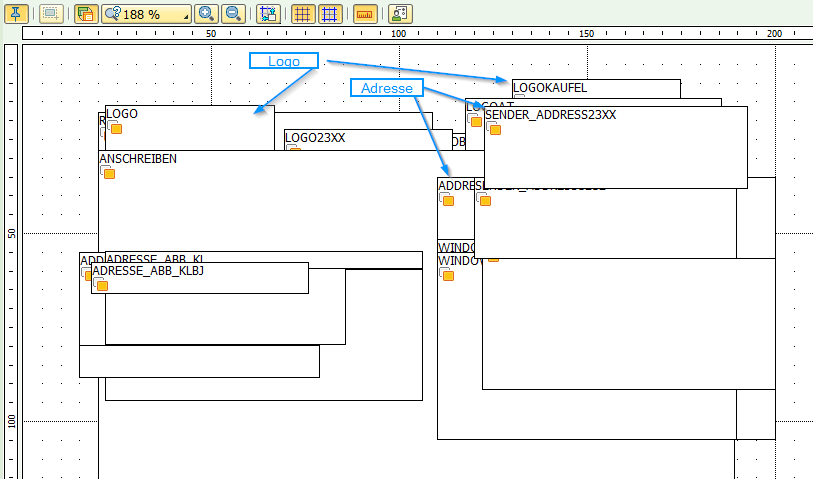
\includegraphics[width=1\textwidth]{img/Smartform-Beispiel-1.png}}%		
		\caption{\ac{LLE} in Smart Forms}
		\label{fig2}
	\end{figure}
	
	Beim Zusammenführen der verschiedenen Varianten des Formulars ein eine Smart Form kam es zusätzlich dazu, dass die verwendeten Texte an unterschiedlichen Stellen hinterlegt wurden. Für den einen Teil der Texte wurden Textbausteine angelegt, welche unabhängig von der Smart Form änderbar sind. Diese Bausteine werden dann im Formular aufgerufen. Der andere Teil der Texte wurde jedoch direkt im Smart Form als Textfeld mit festem Inhalt angelegt. 
	
	Diese Inkonsistenz wird weiter geführt in Form von kleinen \ac{ABAP}-Code Teilen in der Smart Form welche die Formular Daten weiterverarbeiten sowie kleinere Randinformationen zu Verfügung stellen sollen. Diese kleineren Funktionen sind auf das ganze Formular verteilt und oft ist nicht erkennbar, wofür ein kleiner Abschnitt Code zuständig ist.
	

	Diese Punkte sorgen dafür, dass der Änderungsprozess zusätzlich verlängert wird, da bei einem so komplexen Dokument mehr Zeit eingeplant werden muss, da oftmals Mitarbeiter an dem Dokument Änderungen vornehmen müssen ohne das Formular davor schon gekannt zu haben. Ein zusätzlicher Einarbeitungsaufwand ist somit vorhanden.
	
	Grundsätzlich funktioniert die \ac{LLE} in ihrem jetzigen Zustand, aber weitere Änderungen seitens der Zoll-Vorgaben oder seitens der Gesellschaften führen immer mehr zu zusätzlichem Aufwand, welcher bei einer optimierten Lösung nicht nötig wären.
	
	Wie in Abbildung \ref{fig3} zu sehen ist, wird die \ac{LLE} aktuell in drei Sprachen gleichzeitig erstellt. Obwohl es gesetzlich nicht so vorgegeben ist stehen alle drei Sprachen gleichzeitig auf dem Dokument um den zusätzlichen Aufwand einer Übersetzung zu vermeiden.
	
		\begin{figure}[ht]
		\centering
		\makebox[\textwidth][c]{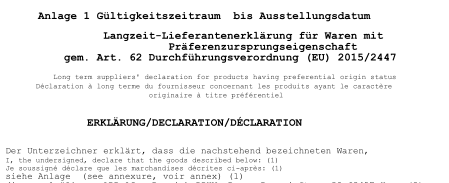
\includegraphics[width=1\textwidth]{img/Sprachen.png}}%		
		\caption{Mehrsprachige \ac{LLE}}
		\label{fig3}
	\end{figure}

	Die Zuweisung eines Formulars zu einer Gesellschaft findet im Customizing statt. Das Customizing ist ein separater Bereich von SAP in welchem Einstellungen, Funktionen und Prozesse gesteuert werden. Im Fall der \ac{LLE} wird hier festgelegt für welche Verwaltungseinheit welches Dokument verwendet wird. In Abbildung \ref{fig4} ist zu sehen, dass bei Smart Forms zusätzlich auch noch ein Formulartext festgelegt werden kann.
	
			
		\begin{figure}
		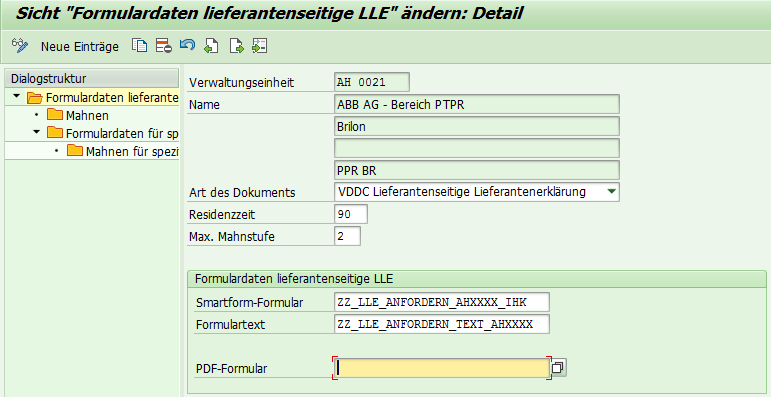
\includegraphics[width=1\textwidth]{img/Customizing.png}	
		\caption{Customizing der \ac{LLE}}
		\label{fig4}
	\end{figure}

	\FloatBarrier

	\section{Anforderungen}
		Die Grundanforderungen an das neue Formular ist, dass am Ende das selbe Dokument ausgedruckt wird wie bei den Smart Forms. Optisch soll kein großer Unterschied für die operativen Einheiten vorhanden sein. Des weiteren ist es sehr wichtig das auch anderweitig die Fachbereiche durch die Umstellung auf Adobe PDFs nicht beeinträchtigt werden.
	
		Gesellschaftsspezifische Inhalte, wie beispielsweise die Logos, sollen weiterhin dynamisch angedruckt werden.
		Die Adressfelder, welche bei den Smartforms unterschiedlich sind, sollen vereinheitlicht werden um das Formular, technisch gesehen, übersichtlicher zu machen. Trotz der Vereinheitlichung sollen trotzdem noch alle Daten angezeigt werden, welche schon jetzt auf dem Formular stehen. 
		
		Um zukünftige Änderungen am Formular einfacher zu machen müssen alle Elemente und Komponenten der Adobe \ac{PDF} einheitlich und leicht verständlich benannt sein. Wird kein System verfolgt bei der Erstellung des Formulars kann es dazu führen das erneut ein erhöhter Einarbeitungsaufwand nötig ist.
		
		Für die \ac{LLE} ist es nicht von Nöten eine optimierte Art der automatischen Übersetzung der Texte zu finden, da alle nötigen Sprachen \footnote{Deutsch, Englisch und Französisch} gleichzeitig im selben Formular aufgedruckt werden.
		Dennoch ist es erforderlich eine konsistente Art der Übersetzung von Formularen zu "finden? " um zukünftige Umstellungen damit zu vereinfachen.
